\documentclass[letterpaper,12pt]{article}
\usepackage{natbib}
\bibliographystyle{unsrtnat}
\usepackage{amsmath}  
\usepackage{graphicx} 
\usepackage[margin=1in,letterpaper]{geometry}
\usepackage{libertine}
\usepackage[final]{hyperref}
\hypersetup{
	colorlinks=true,      
	linkcolor=blue,       
	citecolor=blue,        
	filecolor=magenta,
	urlcolor=blue         
}
\usepackage{titlesec}

\titleformat{\section}{\flushleft\bfseries\Large}{\thesection}{1em}{}

\linespread{1.5}

\begin{document}

\title{FORT: A DeFi Development and Application System with Unlimited Liquidity}
\author{Zaugust \\ James Zhao}
\date{09-09-2021}
\maketitle

\noindent Liquidity is the key to on-chain applications. 
To solve this problem, previously DeFi has tried the traditional idea of order book and Automated Market Maker (AMM) models. 
However, these models are not ideal solutions and cannot integrate all financial services into the same protocol and share the same liquidity, resulting in wasted resources and low performance. 
This paper proposes a new model: FORT protocol, which creates the concept of discounted computers and on-chain currency units, and systematically solves the liquidity and uniformity problem of all DeFi. 
It can be used for all financial product development and economic relationship lock-in of off-chain activities.

\section{History of DeFi}

Decentralized finance, as known as DeFi, is the fastest growing application in the blockchain world and it has found a real demand. 
The history of DeFi can be traced back to the early days of orderbook-based on-chain transactions, as well as peer-to-peer lending.  
Some applications gained attention around 2017, but due to the extremely high cost of on-chain brokering and the lack of a decentralized oracle, this group of projects did not grow. 
Instead, decentralized exchanges (e.g., Uniswap) based on the AMM mechanism and lending protocols (e.g., Compound, MakerDAO) based on liquidity pools and asset prices, grew rapidly and led to the wave of DeFi in 2020. 
Because this type of project better solves the fundamental contradiction of DeFi: lack of on-chain liquidity.

However, whether it is AMM or liquidity pools, the solution to liquidity problems is at the expense of the seller's flexibility: the seller needs to fix his own trading strategy and bear the fluctuations in the external market. 
Once the price is favorable to the seller, the buyer opts out of the deal. Once there is arbitrage, the buyers flock in. 
The seller has no choice but hope for subsidies from mining and commission or interest rate equalization. 
Although this asymmetric design temporarily alleviates the lack of on-chain liquidity, there are the following problems in the long run. 


Firstly, a large amount of assets is occupied and staked in DeFi protocols but only a small number of transactions are supported, resulting in a waste of resources. Most of the total value locked (TVL) is still rushing to liquidity mining for profits. 
In the long term, the lower the capital utilization rate, the greater the loss of intrinsic value of the DeFi products.
Secondly, the core variables, such as asset price and interest rate, are related to the size of the pool, which is easy to be arbitraged on the one hand, and it is difficult to attract many trading and lending users when the pool is not large enough on the other hand. 
Moreover, TVL of various DeFi products cannot be shared, resulting in the composability of DeFi products only at the technical calling level, rather than liquidity sharing.

This kind of liquidity created at the expense of one party's choice is not a perfect idea under a decentralized architecture. 
Instead of allowing the seller to make asymmetric sacrifices, it is better to completely erase this asymmetry. 
The system only allows a completely symmetric buyer, and the seller is the system itself. 
This idea complies with the decentralized game spirit of the blockchain. 
Everyone is in the same position to play the game, whether it is Bitcoin or Ethereum. 
Each participant only needs to burn system tokens in consideration to get the financial products they want, and the income of the financial products will be settled by minting system tokens. 
It frees us from the traditional financial trading models and forms a new financial paradigm which not only ensures composability but also renders all DeFi products equivalent to linear transformations in the same framework, with uniform programmability.

\section{FORT Principle}

Financial services or products can be considered as the exchange of future revenue streams and current expenditure streams. 
If we use $S_t$ to denote the price or interest rate information stream, $R_i$ as the revenue stream, $C_i$ as the expenditure stream, and $\mathcal{T}_0$ and $\mathcal{T}_1$ as the time domain of expenditure and revenue respectively, then the diagram of financial services or products is illustrated as follows:

\begin{figure}[h]
\centering
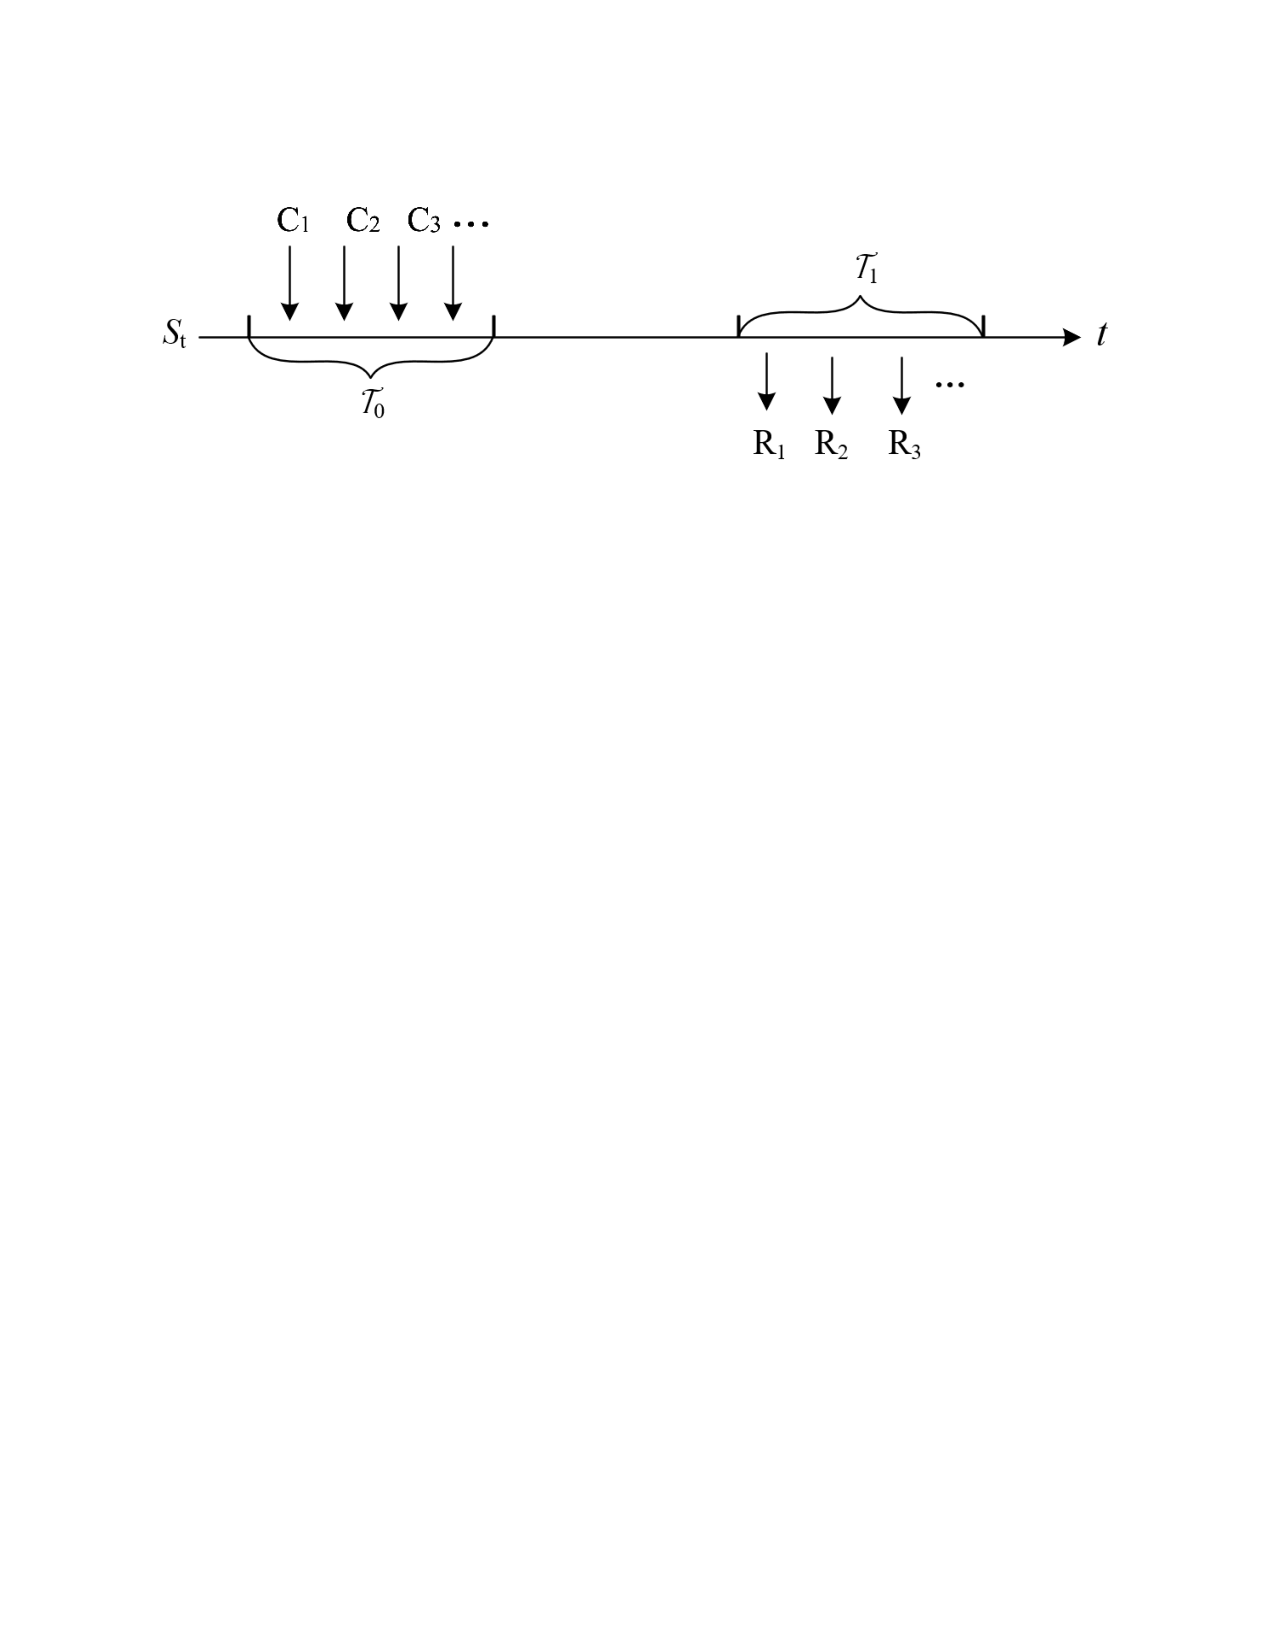
\includegraphics[width=4.5in]{fig-1}
\caption{Diagram of financial services or products}
\end{figure}

The principle of FORT is that, according to a given discounting algorithm, future revenue streams and current expenditure streams are equivalent (or slightly smaller, in this case for deflation), so each revenue stream corresponds to an expenditure stream, and both revenue streams and expenditure streams are uniformly settled with the decentralized currency unit (DCU). 
If we regard the future revenue streams as a financial product, we can call the corresponding expenditure streams the present value or cost of the product. 
We use $r$ to denote the discount rate, and $\mathcal{F}_0$  as the information set at the time of the transaction, this process can be described as following:

\begin{equation}
\sum_{\mathcal{T}_1} E\left[e^{-rt_{i}}R_{i}|\mathcal{F}_0\right] \leq \sum_{\mathcal{T}_0} E\left[e^{-rt_{i}}C_{i}|\mathcal{F}_0\right] 
\label{e1}
\end{equation}

Since a financial product can consist of a linear combination of basic revenue functions (BRF), each of which corresponds to a basic discount function (BDF), the cost of the product is a linear combination of these basic discount functions.
Thus, we can design the basic revenue function and its discount function as a developable model: a discounted computer - any financial product can be developed by this computer, and the basic revenue function is like the instructions of the computer. 
The basic discount function is like the cost of these instructions or EVM-like gas, except that the gas is paid in DCUs, and the instructions produce DCUs. The calculation of the financial product $P$ and its cost $C(P)$ can be described as:

\begin{equation}
P=x_1\cdot BRF_1+x_2\cdot BRF_2+\cdots=\boldsymbol{BRF}\cdot \boldsymbol{X^T}
\end{equation}

\begin{equation} 
C(P)=x_i\cdot BDF_1+x_2\cdot BDF_2+\cdots=\boldsymbol{BDF}\cdot \boldsymbol{X^T}
\end{equation}

\noindent $\boldsymbol{X}$ is the linear combination coefficient of the $\boldsymbol{BRF}$ representation and $\boldsymbol{BDF}$ is the discount function of the $\boldsymbol{BRF}$, where

\begin{equation}
E\left[e^{-rt_{i}}BRF_{i}|\mathcal{F}_0\right] \leq E\left[e^{-rt_{i}}BDF_{i}|\mathcal{F}_0\right] 
\end{equation}

The discounted computer can develop a variety of financial products, including options, perpetuals, leveraged trading, swaps, and lending products, to name just a few, and almost any financial product can be produced.

\subsection{DCU Issuance, Settlement and Pricing}

Decentralized Currency Unit (DCU) is issued by FORT protocol and has an unlimited supply, with the initial DCU offering of no more than 100 million. In FORT protocol, DCU is the only settlement currency.
For example, in the future, you will get 300 DCUs if you meet certain conditions, so you need to spend and burn 50 DCUs now, and after 300000 blocks, you will get 300 DCUs minted by the system.

As you can see, all DCU holders share the risks and benefits of DCU issuance or destruction and participate in the equilibrium of supply and demand in the secondary market for DCUs: the demand for DCUs is from those who buy financial products on the chain and invest in DCUs, while the supply is determined by the initial offering and the DCUs settled by the FORT protocol. The advantage of sharing the same settlement unit is that we can build all financial services such as trading, lending, derivatives without issuing too many tokens through continuously improving the liquidity of DCUs.

According to
\begin{equation}
E\left[e^{-rt}BRF|\mathcal{F}_0\right] \leq E\left[e^{-rt}BDF|\mathcal{F}_0\right] 
\end{equation}

Total supply $G_t$ satisfies: 

\begin{equation} 
EG_{t_2} \leq EG_{t_1}, \quad t_2 \geq t_1 
\end{equation}

Total demand ($D_t$) is determined by trading demand, and the price of DCUs ($P_t$) is determined by the equilibrium of $(D_t, G_t)$. 
Considering the growth of demand and the long-term deflationary nature of supply, there is a logic for a sustained rise in $P_t$

As the DCU is named, combined with FORT contracts, it is an on-chain universal currency with scenarios, which BTC and ETH cannot achieve: BTC has no on-chain scenarios with fixed issuance, ETH follows all scenarios as gas, but its issuance is according to a fixed algorithm, not incremental according to scenarios. DCU is guaranteed to clear in every scenario, which matches the completely decentralized currency envisioned by many economists, and is a further development after BTC-ETH.

\subsection{NEST Oracle}

NEST oracle is the only truly decentralized oracle on the market today: given an off-chain price stream, how to design a decentralized game such that the game equilibrium can output a price stream with the smallest possible deviation from the off-chain price stream. NEST oracle solves this problem with quotation mining, two-way options, validation cycles, price chains and $\beta$ factors.
NEST provides a price sequence that does not change the distribution of asset prices, but approaches a discrete sampling model, which is determined by the structure of the decentralized game, where the quote deviation and quotation density depend on the depth of the arbitrage market and the price of the NEST token. Overall, NEST provides an efficient decentralized oracle that maintains the fundamental traits of asset prices.

In FORT, we tend to use highly efficient market prices, and hence choose the most liquid underlying assets such as BTC and ETH, etc. The basic price model follows the Geometric Brownian Motion (GBM) model. Considering the characteristics of prices deviation and discrete time, we correct the prices using the $k$-factor.

\begin{equation} 
K =(0.00002 * T + 4 * \sigma) * \gamma(\sigma)
\end{equation}
where $\sigma$ is the volatility in seconds and $T$ is the time delay derived from the difference between the height of the successfully packed block and the height of the block where the most recent valid NEST price multiplied by the block time interval, and $\gamma$ takes a value satisfying:

\begin{equation} 
\gamma =\begin{cases}1,\qquad \sigma \leq 0.0003\\
1.5,\quad 0.0003 <\sigma \leq 0.0005\\
2,\qquad \sigma  >0.0005\end{cases}
\end{equation}

\subsection{Time Domain}

The time domain is denoted by $\mathcal{T}_i$ and can be moments or intervals. 
A moment can be a definite moment or a random moment (e.g., a stoppage), and in finance, an interval is often used to determine some mean or stoppage. 
Although the time on the blockchain is discrete, these discrete differences can be ignored for a longer period and compensated for in a shorter period based on the $k$-factor, and thus can be interpreted approximately in terms of continuous time intervals.

\subsection{Discounted Computers}

We abstract all financial products (services) as an exchange of revenue streams and expenditure streams, and the revenue streams are represented by linear combinations of the basic revenue functions. 
Then any financial product development only needs to determine the linear combination of basic revenue functions to obtain its cost (present value) by the linear combination of basic discount functions. 
Such linear combinations are the same as we use computer programming, therefore we call this figuratively as the discounted computer.
Any financial product corresponds to a piece of computer programming, so that the composable DeFi become program designing and calling in the same framework, reducing the difficulty of understanding and risk management.

\subsection{Basic Revenue Function and Discount Function}

The basic revenue function (BRF) can be a deterministic value (e.g., block 13678933 to get 1000 DCUs) or it can be a random variable after introducing the NEST oracle price information. 
Here, we consider the basic types of deterministic values, random variables of NEST pricing oracle, and probability random variables, each of which consists of polynomial functions, exponential functions, logarithmic functions, absolute value functions, maximum-minimum functions, and definite integral operators. 
The base discount function (BDF) contains normal distribution functions, polynomial functions, exponential functions, logarithmic functions, etc. 
Considering that the reality does not need so many revenue functions as well as the complexity of the calculation, we choose a relatively simple list of functions, which can be gradually improved later.
As mentioned earlier, the basic revenue function is the basic instructions of the discounted computer while a financial product is a program which is a combination of these instructions.

\subsection{Discount Rate and Interest Rate Oracle}

In principle, the discount rate reflects the risk-free return of the on-chain world. 
We can choose a risk-free interest rate statistic on the chain such as the PoS yield of ETH or the decentralized interest rate oracle (a design as follows: given the number of DCU issues per year, anyone who locks DCUs can share these tokens proportionally) as the discount rate. 
However, this paradigm is more suitable for a traditional centralized world. In a decentralized world, we can take the discount rate to a relatively small value, even zero, in order to give the DCU deflationary properties and thus ensure a steady rise in the DCU price.

\subsection{Pricing Unit Transformation}

If a fiat or ETH is required as the numeraire in FORT, it is sufficient to introduce the DCU/USDT or DCU/ETH price, which can be obtained through the NEST oracle. If the liquidity of DCU is large enough that the settlement of a single financial product has little impact on the price, the financial product with the introduced price is no different from the traditional financial product. The pricing based on the risk-neutral measure ($E^Q$) can perfectly solve the calculation of the discount function, which can be used for hedging or asset portfolio management.

\begin{equation}
E^Q\left[e^{-rt_{i}}BRF_{i}|\mathcal{F}_0\right] \leq E^Q\left[e^{-rt_{i}}BDF_{i}|\mathcal{F}_0\right] 
\end{equation}

\subsection{Financial Product Development}

The development of a financial product in FORT is the same as writing smart contracts, i.e., finding a vector with BRF as the base for the target return, and that vector represents this financial product. 
The product of that vector and the corresponding BDF base is the cost of the financial product, i.e., it is only necessary to pay this cost in the time domain $\mathcal{T}_0$ to obtain the financial product. 
That financial product will get the DCUs minted by the FORT contract in the time domain $\mathcal{T}_1$, and its quantity is the product of that vector and the BRF.
This process is just like writing smart contracts by which all financial products can be implemented with the discounted computer programming of FORT. 
Developers do not have to operate the liquidity of tokens, and just need the DCUs to be liquid enough.

\section{Applications}

FORT has a wide range of applications, covering almost all financial services and different trading structures (including peer-to-peer, many-to-many, etc.). 
It is a revolutionary design in the history of blockchains, and having the ability of lock-in various off-chain economic relationships.

\subsection{Options and Options Coins}

Options products become pretty simple: giving an expiration date and an exercise price, users can obtain a call or put option whose cost is determined by discount functions. 
Although this formula is not a risk-neutral measure when DCU price is not quoted, so care needs to be taken to understand the implications. 
When the DCU price is quoted, it is the same as traditional options, except that the interaction becomes much simpler and there is not much brokering to consider.

A better model is to issue the options as a token, i.e., the same token for a given expiration date and strike price, regardless of when the issue starts. 
The advantage of this model is that it allows traditional derivatives exchanges to dispense with the issue and settlement. 
In order to meet the issue demand, they either need to do a lot of matchmaking or find a market maker, and in order to settle, they often need margin management. 
Market makers also need to develop a hedging strategy, which is a huge financial auxiliary system. 
Although traditional finance is happy to do so, but its cost is much higher than the FORT model. 
Because the issuance and settlement of the FORT model, exchanges only need to solve the problem of secondary market trading of derivatives.

\subsection{Perpetual Contracts, Leveraged Trading and Leveraged Coins}

Perpetual contracts or leveraged trading can also be very simple, which is a dynamic settlement model based on basic revenue functions. 
We can develop perpetual or leveraged transactions into a model called a leveraged coin: dynamically changing the balance of its tokens based on prices, which has been practiced in current algorithmic stablecoins.

\subsection{Trading, Price Coins and Stablecoins}

A native asset is actually equal to a price coin $*$ DCU, which is equivalent to splitting an asset into a dynamic price and a fixed settlement unit. 
This model can only be effectively implemented in a fully decentralized world: the traditional centralized world has the credit risk of cashing out. 
Thus, trading is equivalent to exchanging DCUs for various price coins, or settling out of DCUs with various price coins. 
Or using the native asset to exchange the corresponding price coin at a ratio of 1 to 1 (which is actually slightly off, due to the price deviation of oracles). 
By analogy, a stablecoin pegged to a fiat currency such as the US dollar is a USDT price coin.

\subsection{Exponential and Logarithmic Coins}

A new paradigm is the exponential coin, where the percentage of price fluctuations feeds into the growth of returns in an exponential manner. 
Compared to leveraged coins, exponential coins have many advantages: no need to close positions, faster growth,  interchangeable transfers, free stacking at the same address, etc. 
For example, when the price doubles, the exponential coin with the e base can grow 7.4 times, and when the price triples, the exponential coin grows 20 times.

\subsection{Revenue Swaps}

Revenue swaps are cost swaps, as they are all equivalent to discounted of revenue streams.

\subsection{Lending}

Lending becomes much easier by pledging asset accepted by FORT to receive the corresponding DCUs, repaying it to receive the collateralized asset, and then being liquidated when the liquidation ratio is exceeded, where the core parameters are the liquidation ratio, collateral rate, interest rate, etc.

\subsection{Insurance}

Based on the characteristics at the end of the event, a price insurance can be made to swap the loss with the premium.

\subsection{Interest Rate Derivatives}

It is possible to design various interest rate derivatives through price information of the base interest rate oracle.

\subsection{Probability Coins}

Design probability coins that get DCUs at a given moment with a predetermined probability. For example, coins with 1/10 probability, each probability coin have a 1/10 probability of getting 10 DCUs.

\subsection{NFT Applications}

It is possible to lock in all economic relationships in off-chain games or NFTs based on DCU, i.e. all game assets can be designed to some probability coins or derivatives above. 
In this way, its game assets corresponding to NFT can be cashed in FORT, regardless of the existence of that game, thus building a consistent variable in the game world.

\subsection{Multi-Party Trading}

To design a transaction between two or more participants: A and B can create a contract based on FORT, each paying a certain amount of DCUs at the current moment and receiving the corresponding DCUs in the future, so that FORT can participate in the allocation between them, which realizes a multi-player competition and game structure.

\section{Summary}

FORT offers a new paradigm: financial products are considered as programming over basic discount functions. 
The cost is the expense of calling those functions, just like EVM. The difference is that the economic relations of the discounted computer are inherent. 
The new paradigm can cover almost all financial products (services) which can be bought at any time and settled with unlimited liquidity, where market makers, margin (call), and fear of being unable to settle are not required. 
As long as the DCU liquidity is sufficient, it would be extremely easy to recreate the traditional financial market. 
Moreover, as difficulties of issuance and settlement are solved, traditional derivatives exchanges can focus on the secondary market, thus significantly reducing their costs. 
In addition, FORT can bring the fundamental consistent variables for the metaverse, with the ability to traverse different games to lock in economic relationships.

\bibliography{ref}

\end{document}
